\documentclass[12pt,a4paper,2sides]{report}
\usepackage{lib/lib} %import libary from lib.sty %
%Thêm thư viện ở dưới dòng này.
\usepackage{float}

\usepackage{graphicx}
\usepackage{tikz}
\usetikzlibrary{positioning}
\usetikzlibrary{arrows.meta}
\usepackage{amsmath}
\usepackage{graphicx}
\usepackage{caption}
\usepackage{subcaption}
\usepackage{booktabs}

\onehalfspacing %Giãn dòng phân nửa.
%===============================
%Thêm dữ liệu vào intro.tex qua dòng lệnh.
%Addition into data at intro.tex file via command.
\newcommand{\khoa}{Information Technology} %TÊN NGÀNH, KHOA.
\newcommand{\de}{Detecting Fraud in Online Payments with Graph Neural Networks}
\newcommand{\monhoc}{Research Topics 1} %TÊN MÔN HỌC 
\newcommand{\chuyennganh}{Computer Science}
\newcommand{\gvhd}{PhD. Le Van Vang} %TÊN CỦA GIẢNG VIÊN HƯỚNG DẪN
\newcommand{\tacgia}{Bui Huu Loc - 521H0504} %TÊN CỦA NGƯỜI VIẾT
\newcommand{\nam}{2024}
%Acknowledge page (the second page in docs)
% \newcommand{\loicamon}{
% 		Với những kiến thức em tích lũy được qua những ngày học tập, đây là kết quả của quá trình học tập của em và nhóm cùng đưa ra ý kiến và thảo luận, tổng hợp kiến thức lại với nhau.\\
% }
%tabl

\begin{document}	
\pagenumbering{roman}

\pagenumbering{gobble}
\begin{center}
	\large{\textbf{VIETNAM GENERAL CONFEDERATION OF LABOUR}} \\
	\large{\textbf{TON DUC THANG UNIVERSITY}} \\
	\large{\textbf{\MakeUppercase{FACULTY OF \khoa}}} \\\vspace*{1cm}	
	\includegraphics[width=0.5\linewidth]{lib/TDTlogo.jpg}\\\vspace*{1cm}	
	
	\large{\textbf{\tacgia}}\\\vspace*{1.5cm}
	

	\LARGE{\textbf{\MakeUppercase{Detecting Fraud in \\ Online Payments with \\Graph Neural Networks}}}\\\vspace*{1.5cm}
	
	\LARGE{\textbf{\MakeUppercase{\chuyennganh}}}\\\vspace*{1.5cm}
	
	\Large{\textbf{\MakeUppercase{\monhoc}}}\vspace*{1.5cm}

	\large{\textbf{Ho Chi Minh City, \nam.}}
\end{center}
\newpage
\include{cover2}
\newpage
\pagenumbering{roman}
\setcounter{page}{1}
\begin{center}
	\Large{\textbf{ACKNOWLEDGEMENT}}
\end{center}

	I would like to thank the lecturer \gvhd \mbox{} for enthusiastically teaching and helping me in completing the exercises, as well as understanding the issues of the subject.\\
	
	With the knowledge I have accumulated through my days of study, this is the result of my learning process. Although there are still many limitations, I will try to achieve the best results possible.\\
	\newpage
\begin{center}
	\Large{\textbf{ESSAY COMPLETED}} \\
	\Large{\textbf{AT TON DUC THANG UNIVERSITY}} \\
\end{center}

I declare that this product report is mine alone. The research content and results in this topic are honest and have not been published in any form. The data in the tables for analysis, comments, and evaluation were collected by the author from different sources and clearly stated in the reference section.\\

In addition, the topic also uses a number of comments, assessments as well as data from other authors and other organizations, all with clear and specific citations and annotations of the origin.\\

If any fraud is discovered, I will take full responsibility for the content of the article. Ton Duc Thang University is not involved in copyright violations during my work.\\

\begin{center}
	\hspace*{7cm}Ton Duc Thang University,\\
	\hspace*{7cm}22 March \nam.\\
	\hspace*{7cm}Students perform,\\
	\hspace*{7cm}(Sign and write full name)\\
	\vspace*{0.2cm}
	\vspace*{2cm}
	 %\includegraphics[width=0.7\linewidth]{lib/signate.png}\\
	\hspace*{7cm}\tacgia.
\end{center}		

\newpage
\begin{center}
	\Large{\textbf{Detecting Fraud in Online Payments with \\Graph Neural Networks}} \\
\end{center}
\hspace{\parindent}
Fraudulent activities in online payment systems pose significant risks to both businesses and consumers. Traditional fraud detection methods often struggle to adapt to the evolving nature of fraudulent tactics and the increasing volume of transactions. In this study, we propose a novel approach leveraging Graph Neural Networks (GNNs) for fraud detection in online payments. By modeling transaction data as a graph, we capture intricate relationships and dependencies between transactions, enabling more effective detection of anomalous behavior indicative of fraud. We explore the development and implementation of this approach, along with potential avenues for further improvement. Our findings suggest that utilizing GNNs for fraud detection offers promising results and opens up new opportunities for enhancing security in online payment systems.

\newpage
\begin{center}
	\Large{\textbf{CONFIRMATION AND EVALUATION SECTION}}
\end{center}
	\textbf{Evaluation by the instructor marking the test:}\\
	...............................................................................................................................................\\
	...............................................................................................................................................\\
	...............................................................................................................................................\\
	...............................................................................................................................................\\
	...............................................................................................................................................\\
	...............................................................................................................................................\\
	...............................................................................................................................................\\
	...............................................................................................................................................\\
	...............................................................................................................................................
\begin{center}
	\hspace*{5cm} Ho Chi Minh city, 22 March \nam.\\
	\hspace*{5cm} Instructor grades papers,\\
	\vspace*{1.2cm}
	\hspace*{5cm} .......................................
\end{center}
	\vspace*{0.5cm}
	\textbf{Instructor's evaluation section:}\\
	...............................................................................................................................................\\
	...............................................................................................................................................\\
	...............................................................................................................................................\\
	...............................................................................................................................................\\
	...............................................................................................................................................\\
	...............................................................................................................................................\\
	...............................................................................................................................................\\
	...............................................................................................................................................\\
	...............................................................................................................................................
\begin{center}
	\hspace*{5cm} Ho Chi Minh City, 22 March \nam.\\
	\hspace*{5cm} Instructor guides,\\
	\vspace*{2cm}
	\hspace*{5cm} \gvhd.
\newpage
\end{center}


\newpage
\clearpage
%--------------Mục lục
\dominitoc
\tableofcontents %pages
%if you want to show table of contents of chapter, set \dominitoc under line \chapter{name}
%\listoffigures %pictures
\listoftables
\listoffigures
\newpage
\clearpage

%\setcounter{page}{-1}
%\listoftables
%\begin{figure/tables}
%\centering
%Sourcode/Import
%\caption
%\end{fugure/tables}
\clearpage
\pagenumbering{arabic}
\setcounter{page}{1}
\clearpage
%\Control to file to create subfile.\\
%\input{part1.tex}

% chapter 1
\chapter{Introduction}
\section{Background and Motivation}
\hspace{\parindent}
In recent years, the proliferation of online transactions has led to an exponential increase in the volume of digital payments worldwide. While this surge in digital commerce has revolutionized the way we conduct business, it has also opened new avenues for fraudulent activities. According to recent studies, online payment fraud is estimated to cost businesses billions of dollars annually, posing significant financial losses and reputational damage.\\

Traditional fraud detection methods, primarily based on rule-based systems and static thresholds, have become inadequate in dealing with the sophisticated tactics employed by fraudsters. These methods often struggle to adapt to evolving fraud patterns and struggle to distinguish between legitimate and fraudulent transactions accurately.\\

To address these challenges, there has been a growing interest in leveraging advanced machine learning techniques, particularly Graph Neural Networks (GNNs), for fraud detection in online payments. GNNs offer a promising approach by modeling the complex relationships and interactions inherent in payment networks, thus capturing the intricate patterns indicative of fraudulent behavior.\\

The motivation behind this project stems from the need to develop more robust and adaptive fraud detection systems capable of mitigating the risks associated with online payments. By harnessing the power of GNNs, we aim to enhance the accuracy and efficiency of fraud detection while minimizing false positives and false negatives. Ultimately, our goal is to contribute to the development of scalable, data-driven solutions that can effectively combat fraudulent activities in online transactions.\\

In this report, we present our approach to detecting fraud in online payments using Graph Neural Networks. We delve into the methodology employed, the dataset utilized, the experimental results obtained, and the implications of our findings. Through this research endeavor, we seek to provide insights into the potential of GNNs in bolstering the security and integrity of digital payment ecosystems.\\

\section{Objectives of the Project}
\hspace{\parindent}
Developing a Fraud Detection System: The foremost objective is to design and implement a robust fraud detection system tailored specifically for online payment networks. This system will leverage Graph Neural Networks (GNNs) to effectively capture the complex relationships and patterns indicative of fraudulent behavior within the payment ecosystem.\\

Exploring Graph Representation: We aim to explore various methods of representing online payment networks as graphs, including node and edge attributes, graph construction techniques, and feature engineering. By representing the payment data in a graph structure, we seek to exploit the inherent relational information to enhance the accuracy of fraud detection.\\

Utilizing Graph Neural Networks: The project aims to investigate the effectiveness of Graph Neural Networks in detecting fraudulent transactions within online payment networks. We will explore different GNN architectures, including graph convolutional networks (GCNs) and graph attention networks (GATs), to identify the most suitable model for our specific use case.\\

Training and Evaluation: Our objective is to develop robust training strategies for the GNN-based fraud detection system, including data preprocessing, model training, and validation techniques. We will also establish comprehensive evaluation metrics to assess the performance of the system accurately.\\

Performance Benchmarking: Another objective is to benchmark the performance of the proposed GNN-based fraud detection system against traditional machine learning approaches and baseline models. By conducting comparative analyses, we aim to demonstrate the superiority of GNNs in detecting fraudulent activities in online payments.\\



% chapter 2
\chapter{Literature Review}
\section{Previous approaches to fraud detection in online payments}
\hspace{\parindent}
Over the years, various approaches have been employed to detect fraudulent activities in online payments. These approaches range from traditional rule-based systems to more sophisticated machine learning algorithms. While each approach has its strengths and limitations, they collectively contribute to the ongoing efforts to combat fraud in the digital payment ecosystem.\\

\subsection{Rule-based Systems}
\hspace{\parindent}
Static Thresholds: One of the earliest methods for fraud detection involved setting static thresholds on specific transaction attributes, such as transaction amount or frequency. Transactions exceeding these thresholds are flagged as potentially fraudulent. However, static thresholds are often rigid and fail to adapt to changing fraud patterns, leading to high false positive rates and missed fraud instances.

Heuristics and Business Rules: Rule-based systems may incorporate domain-specific heuristics and business rules to identify suspicious transactions. These rules are typically based on expert knowledge and historical fraud patterns. While effective in some cases, these rules may not capture all instances of fraud and can be circumvented by sophisticated fraudsters.

\subsection{Supervised Machine Learning}
\hspace{\parindent}
Classification Algorithms: Supervised machine learning algorithms, such as logistic regression, decision trees, and random forests, have been widely used for fraud detection in online payments. These algorithms learn to classify transactions as either legitimate or fraudulent based on labeled training data. While effective in capturing known fraud patterns, supervised methods may struggle to generalize to new and evolving fraud tactics.

Feature Engineering: Feature engineering plays a crucial role in supervised fraud detection systems, where relevant features extracted from transaction data are used as input to the learning algorithms. Common features include transaction amount, location, device information, and user behavior patterns. However, manually crafting informative features can be labor-intensive and may not capture all relevant aspects of fraud.

\subsection{Anomaly Detection}
\hspace{\parindent}
Unsupervised Learning: Anomaly detection techniques aim to identify deviations from normal behavior without relying on labeled training data. Unsupervised learning algorithms, such as clustering and density estimation, are often used to detect anomalous transactions. These algorithms flag transactions that significantly differ from the majority of transactions in terms of their features or patterns. While unsupervised methods can detect previously unseen fraud patterns, they may also generate false alarms for legitimate transactions with uncommon characteristics.

Semi-supervised Learning: Semi-supervised approaches combine elements of supervised and unsupervised learning, leveraging both labeled and unlabeled data to detect anomalies. These methods can learn from both known instances of fraud and normal behavior, enhancing their ability to detect subtle and evolving fraud patterns. However, semi-supervised approaches may require large amounts of labeled data to achieve satisfactory performance.

\subsection{Feature Engineering and Transaction Profiling}
\hspace{\parindent}
Feature Engineering: Feature engineering involves selecting and transforming relevant features from transaction data to improve model performance. Features such as transaction amount, frequency, location, device information, and user behavior patterns can provide valuable insights into fraudulent activity.

Transaction Profiling: Transaction profiling techniques analyze historical transaction data to create profiles or behavior patterns for individual users or entities. Deviations from these profiles can be indicative of fraudulent behavior and used as signals for fraud detection.

\subsection{Deep Learning Approaches}
\hspace{\parindent}
Neural Networks: Deep neural networks, including feedforward neural networks, recurrent neural networks (RNNs), and convolutional neural networks (CNNs), have been applied to fraud detection tasks. These models can automatically learn hierarchical representations from raw transaction data, capturing complex patterns and relationships.

Autoencoders: Autoencoder neural networks are unsupervised learning models that learn to reconstruct input data. They can be used for anomaly detection by training on normal transaction data and identifying instances where the reconstruction error is high, indicating potential fraud.


% chapter 3
\chapter{Theoretical Basis}
\section{Basic graph theory}
\subsection{Graph, vertex and edge}
\hspace{\parindent}
A graph G consists of a set of vertices V and a set of edges E, where each edge connects two vertices. Mathematically, we represent a graph as G=(V,E).

A vertex (plural: vertices) is a fundamental unit of a graph, represented as a point. In applications, vertices often represent entities such as people, cities, or computers.

An edge is a connection between two vertices. It can be directed (pointing from one vertex to another) or undirected (bi-directional). Edges often represent relationships or interactions between entities.

\begin{figure}[H]
  \centering
  \includegraphics[width=0.4\linewidth]{graph.png}
  \caption{Graph}
  \label{fig:usecase}
\end{figure}

\subsection{Undirected Graph and Directed Graph}
\hspace{\parindent}
A directed graph (or digraph) is a graph where each edge has a direction associated with it. In a directed graph, edges are represented as ordered pairs of vertices.

An undirected graph is a graph where edges do not have any direction associated with them. In an undirected graph, edges are represented as unordered pairs of vertices.

\begin{figure}[H]
  \centering
  \includegraphics[width=0.4\linewidth]{Undirected-graph-and-b-directed-graph.png}
  \caption{Undirected Graph and Directed Graph}
  \label{fig:usecase}
\end{figure}


\subsection{Degree, path and cycle}
\hspace{\parindent}
The degree of a vertex is the number of edges incident to it. In a directed graph, we can define in-degree (number of incoming edges) and out-degree (number of outgoing edges) for each vertex.

A path in a graph is a sequence of vertices where each adjacent pair of vertices is connected by an edge. The length of a path is the number of edges it contains.

A cycle in a graph is a path that starts and ends at the same vertex, traversing a sequence of distinct vertices and edges.

\section{Graph Neural Network}
\hspace{\parindent}
A GNN is a transformable function applied to all aspects of a graph (including nodes, edges, and global context) while maintaining the graph's symmetries, such as permutation invariance. It represents a subset of deep learning techniques tailored for analyzing data structured as graphs.

These networks are specifically crafted to operate directly on graph data, offering straightforward solutions for tasks involving predictions at the node, edge, or even entire graph levels.

GNNs excel in tasks where Convolutional Neural Networks (CNNs) encounter limitations.

\subsection{Why do Convolutional Neural Networks (CNNs) fail on graphs?}
\hspace{\parindent}

CNNs are highly effective in tasks such as image classification, recognition, or object detection, where they excel in visualizing and analyzing images.

The core principle of CNNs involves employing hidden convolution and pooling layers to detect spatially localized features using receptive fields in kernel form.

\begin{figure}[H]
  \centering
  \includegraphics[width=0.7\linewidth]{cnn_on_img.png}
  \caption{CNN}
  \label{fig:usecase}
\end{figure}


Convolution operates on images by sliding a window across a two-dimensional grid, applying a function over each window and passing it through multiple layers.

However, generalizing convolution beyond simple two-dimensional grids poses challenges when applied to graphs due to their arbitrary size and complex topology, lacking spatial locality.

Moreover, the unfixed node ordering in graphs complicates CNN operations, as varying node sequences alter the inputs to the network. Graphs necessitate invariant results regardless of node ordering.


\subsection{The simplest GNN}
\hspace{\parindent}
With the numerical representation of graphs constructed using vectors instead of scalars, the groundwork is laid for building a GNN. The initial step involves constructing the simplest GNN architecture, wherein new embeddings are learned for all graph attributes (nodes, edges, global) without utilizing the graph's connectivity.

This GNN employs separate multilayer perceptrons (MLPs) or another preferred differentiable model for each component of the graph, termed as a GNN layer. For every node vector, the MLP is applied to derive a learned node-vector. This process is repeated for each edge to obtain a per-edge embedding, and similarly for the global-context vector, resulting in a single embedding for the entire graph.

\begin{figure}[H]
  \centering
  \includegraphics[width=0.7\linewidth]{basis-gnn.png}
  \caption{A basic Graph Neural Network (GNN) consists of a single layer. It takes a graph as input, and each component (V, E, U) is updated by a Multilayer Perceptron (MLP) to generate a new graph. Each function subscript denotes a distinct function corresponding to a different attribute of the graph at the nth layer of the GNN model.}
  \label{fig:usecase}
\end{figure}

As is customary with neural network modules or layers, these GNN layers can be stacked together.

Since a GNN does not alter the connectivity of the input graph, the output graph of a GNN can be described using the same adjacency list and featuring the same number of vectors as the input graph. However, the output graph contains updated embeddings, reflecting the GNN's adjustments to each node, edge, and global-context representation.



\subsection{GNN Predictions by Pooling Information}
\hspace{\parindent}
Considering the scenario of binary classification, the framework can be extended to the multi-class or regression case. If the task involves making binary predictions on nodes, given that the graph already contains node information, the approach is straightforward - for each node embedding, apply a linear classifier.

\begin{figure}[H]
  \centering
  \includegraphics[width=0.7\linewidth]{chap2/2.png}
  \label{fig:usecase}
\end{figure}

However, it's not always straightforward. For instance, information in the graph might be stored in edges but not in nodes, yet predictions on nodes are required. We need a method to gather information from edges and provide it to nodes for prediction. This can be achieved through pooling. Pooling involves two steps.

\begin{enumerate}
    \item For each item to be pooled, gather each of their embeddings and concatenate them into a matrix.
    \item Aggregate the gathered embeddings, usually through a sum operation.
\end{enumerate}

The pooling operation is represented by the letter p, and gathering information from edges to nodes is denoted as pEn->Vn.

\begin{figure}[H]
  \centering
  \includegraphics[width=0.7\linewidth]{chap2/3.png}
  \label{fig:usecase}
\end{figure}

So, if only edge-level features are available and the goal is to predict binary node information, pooling can be used to route (or pass) information accordingly. The model resembles this structure.

\begin{figure}[H]
  \centering
  \includegraphics[width=0.7\linewidth]{chap2/4.png}
  \label{fig:usecase}
\end{figure}

Similarly, if only node-level features are available and the objective is to predict binary edge-level information, the model takes a similar form.

\begin{figure}[H]
  \centering
  \includegraphics[width=0.7\linewidth]{chap2/5.png}
  \label{fig:usecase}
\end{figure}

When node-level features are available and a binary global property needs to be predicted, all available node information is gathered and aggregated, similar to Global Average Pooling layers in CNNs. The same approach applies to edges.



\begin{figure}[H]
  \centering
  \includegraphics[width=0.7\linewidth]{chap2/6.png}
  \label{fig:usecase}
\end{figure}

In these examples, the classification model c can be replaced with any differentiable model or adapted to multi-class classification using a generalized linear model.


\begin{figure}[H]
  \centering
  \includegraphics[width=0.7\linewidth]{chap2/7.png}
  \label{fig:usecase}
\end{figure}

Now that a simple GNN model has been demonstrated, and binary predictions can be made by routing information between different parts of the graph, this pooling technique serves as a fundamental building block for constructing more advanced GNN models. If new graph attributes are introduced, defining how to pass information from one attribute to another is all that's required.

It's noteworthy that in this simplest GNN formulation, the connectivity of the graph is not utilized within the GNN layer. Each node, edge, and global context is processed independently, with connectivity only used when pooling information for prediction.









% chapter 4
\chapter{Methodology}
\section{Data reviewing}
\subsection{Data description}
\hspace{\parindent}
The data is from Kaggle. Below is description about the dataset\\

\begin{table}[H]
	\begin{tabular}{|p{3cm}|p{2cm}|p{10cm}|}
		\hline
		\textbf{Attribute} & \textbf{Type} &  \textbf{Description} \\
		\hline
		Step & Numerical & Shows a chunk of time, where each step means one hour. \\
		Type & Categorical & Tells what kind of online action it is. \\
		Amount & Numerical & How much money is being moved in the transaction. \\
		NameOrig & Text & The person who starts the transaction. \\
		OldbalanceOrg & Numerical & The amount of money they had before. \\
		NewbalanceOrig & Numerical & The amount they have after. \\
		NameDest & The Text & person getting the money. \\
		OldbalanceDest & Numerical &How much they had before. \\
		NewbalanceDest & Numerical & How much they have after. \\
		IsFraud & Binary & Says if the transaction is a scam or not. \\
		isFlaggedFraud & Binary & Indicator flagging potentially fraudulent transactions based on specific criteria. \\
		\hline
	\end{tabular}
	\caption{Data description}
	\label{tab:Functional}
\end{table}


\subsection{Check unique values}

\begin{figure}[H]
	\centering
	\includegraphics[width=0.7\linewidth]{chap4/unique_values}
	\caption{Unique Values}
	\label{fig:uniquevalues}
\end{figure}

\begin{itemize}
	\item Step: The 'step' column has 743 unique values, which seems reasonable if it represents a discrete time step. The percentage of unique values is extremely low (0.0117\%), indicating that the 'step' values are quite distributed or densely packed.
	\item Type: The 'type' column has 5 unique values, which could represent different types of financial transactions. The percentage of unique values is very low (7.86e-05\%), indicating that the 'type' values are relatively evenly distributed.
	\item Amount: The 'amount' column has a large number of unique values (5,316,900), which is expected as it represents the monetary amount of transactions. The percentage of unique values is high (83.56\%), suggesting a wide range of transaction amounts.
	\item NameOrig: The 'nameOrig' column has a very high number of unique values (6,353,307), which indicates that each transaction initiator has a unique identifier. The percentage of unique values is almost 100\%, suggesting almost every transaction initiator has a unique identifier.
	\item OldbalanceOrg, NewbalanceOrig, NameDest, OldbalanceDest, NewbalanceDest: These columns all have a significant number of unique values, suggesting diversity in account balances and destination names. The percentages of unique values range from 29\% to 56\%, indicating moderate to high diversity in these columns.
	\item IsFraud, IsFlaggedFraud: These binary columns have only 2 unique values each, which is expected for binary indicators. The percentages of unique values are extremely low (0.0000314\%), indicating that the overwhelming majority of transactions are non-fraudulent and not flagged as fraud.
\end{itemize}

\subsection{Check missing values}

\begin{figure}[H]
	\centering
	\includegraphics[width=0.7\linewidth]{chap4/missing_values}
	\caption{Missing Values}
	\label{fig:missingvalues}
\end{figure}

The dataset seems to be well-prepared, with most columns having no missing values. However, the presence of missing values in the 'amount\_to\_oldbalanceOrg\_ratio' column suggests potential data issues in that specific calculation or input data.\\


\section{Data visualization}

\begin{figure}[H]
	\centering
	\includegraphics[width=0.7\linewidth]{chap4/1}
	\caption{Transfers and cash-outs as dominant contributors, representing 42.4\% and 34.5\% of the total transaction amount respectively. Payments constitute a smaller portion at 2.5\%, while debit transactions have minimal impact. Cash-ins also play a notable role, contributing 20.7\% to the overall transaction volume}
	\label{fig:1}
\end{figure}

\begin{figure}[H]
	\centering
	\includegraphics[width=0.7\linewidth]{chap4/2}
	\caption{Comparison of the distribution of transaction amounts between fraudulent and non-fraudulent transactions, aiding in understanding patterns and differences in transaction behavior}
	\label{fig:2}
\end{figure}

\begin{figure}[H]
	\centering
	\includegraphics[width=0.7\linewidth]{chap4/3}
	\caption{Proportion of Fraud vs. Non-Fraud Transactions}
	\label{fig:3}
\end{figure}

\begin{figure}[H]
	\centering
	\includegraphics[width=0.7\linewidth]{chap4/4}
	\caption{The correlation between numerical features in the dataset, with warmer colors indicating stronger positive correlations and cooler colors representing stronger negative correlations. Values closer to 1 or -1 signify higher correlation, while values closer to 0 indicate weaker correlation. This visualization aids in identifying potential relationships and dependencies between different variables in the dataset}
	\label{fig:4}
\end{figure}



\section{Data preprocessing}
\subsection{Remove null values}
\hspace{\parindent}
The dataset contained null values in one feature, namely \texttt{amount\_to\_oldbalanceOrg\_ratio}. To address this issue, a common approach of filling null values with the mean of the column was employed.


\subsection{Determine transaction direction}
\hspace{\parindent}
A new feature, \texttt{transaction\_direction}, was created to categorize transactions as either outgoing or incoming based on the transaction amount. This binary categorization enhances the dataset by providing insights into the nature of each transaction. Outgoing transactions are labeled as 'Outgoing' if the amount is greater than zero, and 'Incoming' otherwise.

\subsection{Create amount bins}
\hspace{\parindent}
The continuous variable \texttt{amount} was discretized into bins to simplify its representation and potentially capture nonlinear relationships between transaction amounts and other features. The following bins were defined:

\begin{itemize}
	\item Very Low: Amounts between $0$ and $1000$
	\item Low: Amounts between $1000$ and $5000$
	\item Medium: Amounts between $5000$ and $10000$
	\item High: Amounts between $10000$ and $50000$
	\item Very High: Amounts above $50000$
\end{itemize}

These bins were created using the \texttt{cut} function from the \texttt{pandas} library in Python. The resulting discrete variable, \texttt{amount\_bin}, allows for a more straightforward analysis of the transaction amounts and their potential impact on fraud detection.



\subsection{Encode categorical features}
\hspace{\parindent}
Categorical features such as \texttt{nameOrig}, \texttt{nameDest}, \texttt{transaction\_direction}, and \texttt{amount\_bin} were encoded using the LabelEncoder from the scikit-learn library. This preprocessing step converts categorical variables into numerical labels, facilitating their use in machine learning models.


\subsection{Construct Node Features and Edges}
\hspace{\parindent}
Node features and edges were constructed for the graph representation using the provided data. Node features were derived from selected attributes including 'amount', 'oldbalanceOrg', 'newbalanceOrig', 'oldbalanceDest', and 'newbalanceDest', and converted into a torch tensor of type \texttt{float32}.


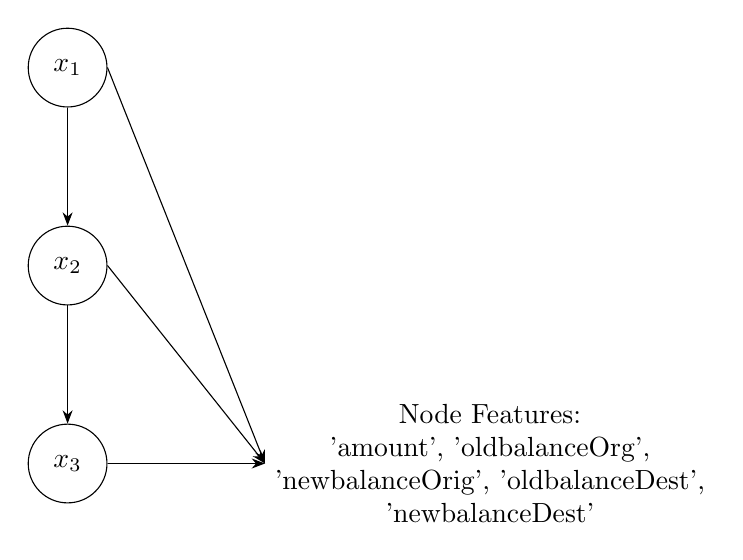
\begin{tikzpicture}[
	node/.style={draw, circle, minimum size=1cm},
	edge/.style={->, >=Stealth}
	]
	% Nodes
	\node[node] (n1) {$x_1$};
	\node[node, below=1.5cm of n1] (n2) {$x_2$};
	\node[node, below=1.5cm of n2] (n3) {$x_3$};
	
	% Node features
	\node[right=2cm of n3, align=center] (features) {Node Features: \\ 'amount', 'oldbalanceOrg', \\ 'newbalanceOrig', 'oldbalanceDest', \\ 'newbalanceDest'};
	
	% Edges
	\draw[edge] (n1) -- (n2);
	\draw[edge] (n2) -- (n3);
	\draw[edge] (n1.east) -- (features.west);
	\draw[edge] (n2.east) -- (features.west);
	\draw[edge] (n3.east) -- (features.west);
\end{tikzpicture}

To establish unique identifiers for nodes, a mapping was created based on the 'node\_identifier' column, ensuring each node has a distinct identifier. The 'nameOrig' and 'nameDest' columns were updated accordingly using the generated mapping.

Edges were defined using the 'nameOrig' and 'nameDest' columns, and converted into a torch tensor of type \texttt{long}, ensuring compatibility with PyTorch. The resulting data structure, \texttt{data}, encapsulates both node features and edge information, facilitating subsequent graph neural network operations.

\begin{figure}[H]
	\centering
	\includegraphics[width=0.7\linewidth]{chap4/5}
	\caption{Visualize the GNN}
	\label{fig:5}
\end{figure}


\section{Graph Neural Network Architecture}
\hspace{\parindent}
The graph neural network (GNN) architecture used for fraud detection in online payments comprises multiple layers of graph convolutional units, each processing information from neighboring nodes within the payment network.

The GNN model consists of two graph convolutional layers (\texttt{GCNConv}), with the first layer transforming input node features to a hidden representation and the second layer further refining the hidden representation to produce the final output.

The \texttt{forward} method of the \texttt{GNNModel} class defines the forward pass of the model. It takes the input graph data, including node features (\texttt{x}) and edge indices (\texttt{edge\_index}), and applies the graph convolutional layers to propagate information through the graph. The ReLU activation function is applied after each convolutional layer to introduce non-linearity to the model.

This architecture leverages graph convolutional operations to capture complex relationships and patterns within the online payment network, enabling effective fraud detection through graph-based learning mechanisms.

\begin{figure}[H]
	\centering
	\resizebox{\textwidth}{!}{%
		\begin{tikzpicture}[
			node/.style={draw, circle, minimum size=1cm},
			layer/.style={draw, rectangle, minimum width=2cm, minimum height=1cm},
			arrow/.style={->, >=Stealth}
			]
			% Input layer
			\node[node] (x1) {$x_1$};
			\node[node, below=0.5cm of x1] (x2) {$x_2$};
			\node[node, below=0.5cm of x2] (x3) {$x_3$};
			\node[node, below=0.5cm of x3] (x4) {$x_4$};
			\node[node, below=0.5cm of x4] (x5) {$x_5$};
			
			% Graph convolutional layers
			\node[layer, right=2cm of x3] (conv1) {Graph Convolutional Layer};
			\node[layer, right=2cm of conv1] (relu1) {ReLU Activation};
			\node[layer, right=2cm of relu1] (conv2) {Graph Convolutional Layer};
			
			% Output layer
			\node[node, right=2cm of conv2] (output) {Output};
			
			% Connections
			\foreach \i in {1,2,3,4,5}
			\draw[arrow] (x\i) -- (conv1);
			\draw[arrow] (conv1) -- (relu1);
			\draw[arrow] (relu1) -- (conv2);
			\draw[arrow] (conv2) -- (output);
		\end{tikzpicture}%
	}
	\caption{Graph Neural Network Architecture}
	\label{fig:gnn_architecture}
\end{figure}

\section{Training the Graph Neural Network}
\hspace{\parindent}
To train the Graph Neural Network (GNN) model for fraud detection in online payments, an optimizer and a loss criterion are defined. The optimizer, instantiated with the Adam optimizer from PyTorch, is utilized to update the parameters of the GNN model during training. Additionally, the CrossEntropyLoss function is employed as the loss criterion to compute the discrepancy between the model predictions and the ground truth labels.

The training process iterates over a fixed number of epochs, during which the optimizer is reset to zero gradients using the optimizer.zero\_grad() method. The output predictions of the GNN model (out) are computed using the forward pass with the input data (data). Subsequently, the loss between the predictions and the target labels is calculated using the defined loss criterion. The gradients are then backpropagated through the network using the loss.backward() method, and the optimizer updates the model parameters using the computed gradients with optimizer.step().

Following the training loop, the GNN model is evaluated on a held-out dataset to obtain node embeddings. The model is set to evaluation mode using gnn\_model.eval() to disable dropout and batch normalization layers that are active during training. Node embeddings are generated by applying the first graph convolutional layer (gnn\_model.conv1) to the input data (data.x) and edge indices (data.edge\_index). The resulting embeddings are detached from the computation graph using .detach() and converted to NumPy arrays for further analysis.


\begin{figure}[htbp]
	\centering
	\resizebox{\textwidth}{!}{%
		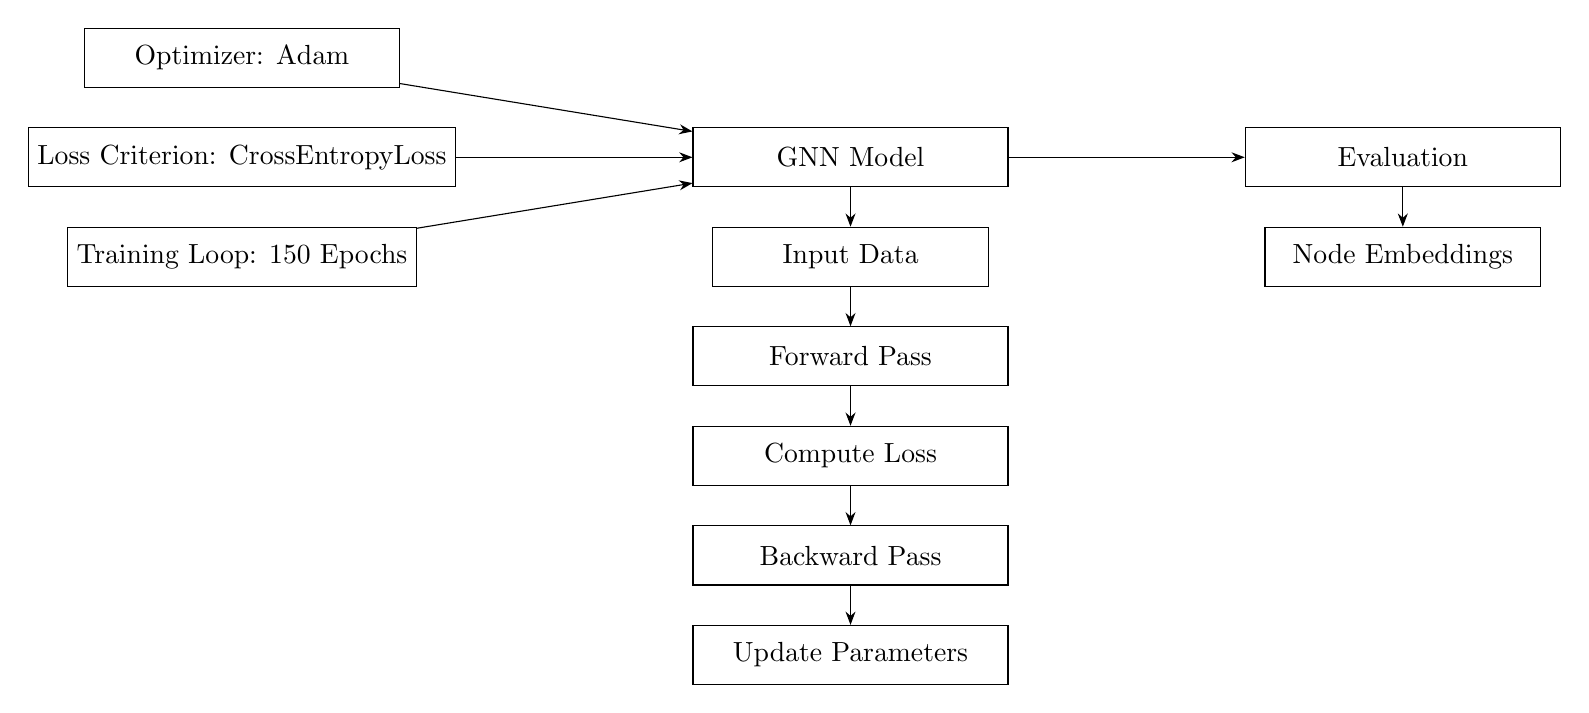
\begin{tikzpicture}[
			node/.style={draw, rectangle, minimum width=3.5cm, minimum height=0.75cm},
			process/.style={draw, rectangle, minimum width=4cm, minimum height=0.75cm, align=center},
			arrow/.style={->, >=Stealth}
			]
			% Nodes
			\node[process] (optimizer) {Optimizer: Adam};
			\node[process, below=0.5cm of optimizer] (criterion) {Loss Criterion: CrossEntropyLoss};
			\node[process, below=0.5cm of criterion] (loop) {Training Loop: 150 Epochs};
			
			% GNN model
			\node[process, right=3cm of criterion] (model) {GNN Model};
			\node[node, below=0.5cm of model] (data) {Input Data};
			\node[process, below=0.5cm of data] (forward) {Forward Pass};
			\node[process, below=0.5cm of forward] (loss) {Compute Loss};
			\node[process, below=0.5cm of loss] (backward) {Backward Pass};
			\node[process, below=0.5cm of backward] (update) {Update Parameters};
			
			% Evaluation
			\node[process, right=3cm of model] (evaluation) {Evaluation};
			\node[node, below=0.5cm of evaluation] (node_embeddings) {Node Embeddings};
			
			% Arrows
			\draw[arrow] (optimizer) -- (model);
			\draw[arrow] (criterion) -- (model);
			\draw[arrow] (loop) -- (model);
			\draw[arrow] (model) -- (data);
			\draw[arrow] (data) -- (forward);
			\draw[arrow] (forward) -- (loss);
			\draw[arrow] (loss) -- (backward);
			\draw[arrow] (backward) -- (update);
			\draw[arrow] (model) -- (evaluation);
			\draw[arrow] (evaluation) -- (node_embeddings);
		\end{tikzpicture}%
	}
	\caption{Training Process for the Graph Neural Network (GNN) Model}
	\label{fig:gnn_training_process}
\end{figure}

\section{Anomaly Detection and Fraud Identification}
\hspace{\parindent}
An Isolation Forest algorithm is utilized for anomaly detection to identify potentially fraudulent transactions within the online payment dataset. Initially, the Isolation Forest model is instantiated without any hyperparameters specified.

Subsequently, the Isolation Forest model is trained using the node embeddings obtained from the previously trained Graph Neural Network (GNN) model. These node embeddings serve as input features for the Isolation Forest algorithm.

Once the Isolation Forest model is trained, anomaly scores are computed for each transaction using the decision\_function() method. These anomaly scores indicate the degree of abnormality of each transaction within the dataset.

A threshold value is then set to classify transactions as potentially fraudulent or non-fraudulent based on their anomaly scores. Transactions with anomaly scores below the threshold are labeled as potentially fraudulent.

Finally, transactions identified as potentially fraudulent are printed to facilitate further investigation and analysis. This provides insights into suspicious transactions that may warrant additional scrutiny for potential fraudulent activity.

\begin{figure}[htbp]
	\centering
	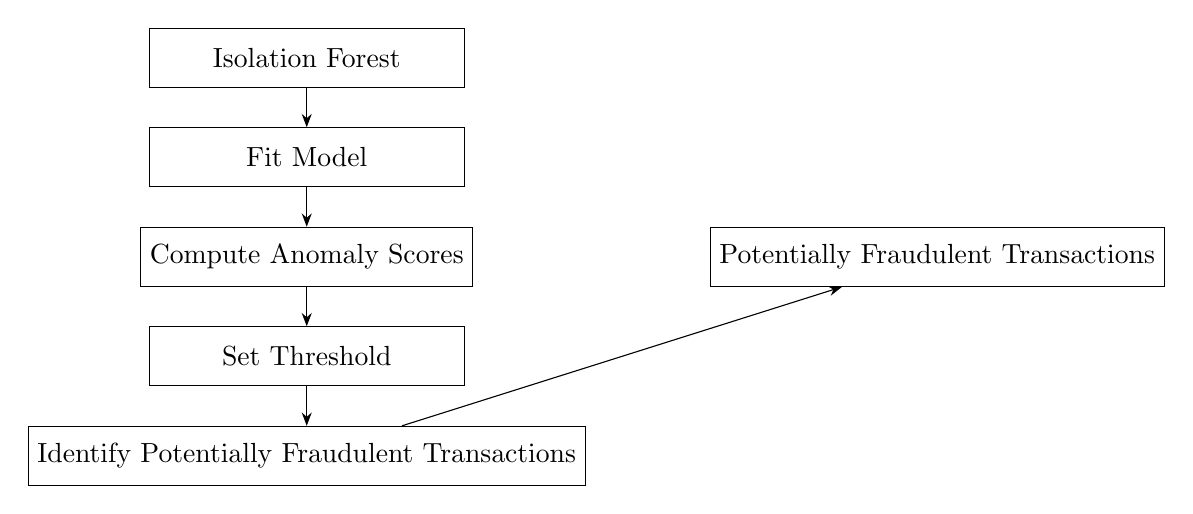
\begin{tikzpicture}[
		node/.style={draw, rectangle, minimum width=3.5cm, minimum height=0.75cm},
		process/.style={draw, rectangle, minimum width=4cm, minimum height=0.75cm, align=center},
		arrow/.style={->, >=Stealth}
		]
		% Nodes
		\node[process] (iso_forest) {Isolation Forest};
		\node[process, below=0.5cm of iso_forest] (fit) {Fit Model};
		\node[process, below=0.5cm of fit] (decision) {Compute Anomaly Scores};
		\node[process, below=0.5cm of decision] (threshold) {Set Threshold};
		\node[process, below=0.5cm of threshold] (identify) {Identify Potentially Fraudulent Transactions};
		
		% Output
		\node[node, right=3cm of decision] (output) {Potentially Fraudulent Transactions};
		
		% Arrows
		\draw[arrow] (iso_forest) -- (fit);
		\draw[arrow] (fit) -- (decision);
		\draw[arrow] (decision) -- (threshold);
		\draw[arrow] (threshold) -- (identify);
		\draw[arrow] (identify) -- (output);
	\end{tikzpicture}
	\caption{Process of Anomaly Detection and Fraud Identification using the Isolation Forest Algorithm}
	\label{fig:anomaly_detection}
\end{figure}


% chapter 5
\chapter{Results and Data Analysis}

\section{Evaluation Metrics}
\hspace{\parindent}
Evaluation metrics to assess the effectiveness of the anomaly detection and fraud identification process:

\begin{itemize}
	\item \textbf{Accuracy}: Measures the overall correctness of the predicted labels compared to the true labels.
	\item \textbf{Precision}: Indicates the proportion of correctly identified potentially fraudulent transactions among all transactions identified as potentially fraudulent.
	\item \textbf{Recall}: Represents the proportion of correctly identified potentially fraudulent transactions among all truly fraudulent transactions.
	\item \textbf{F1 Score}: Harmonic mean of precision and recall, providing a balance between the two metrics.
	\item \textbf{Confusion Matrix}: Provides a detailed breakdown of true positive, false positive, true negative, and false negative predictions.
\end{itemize}


\begin{table}[H]
	\centering
	\caption{Evaluation Metrics}
	\label{tab:results}
	\begin{tabular}{@{}ll@{}}
		\toprule
		Metric      & Value   \\ \midrule
		Accuracy    & 0.9803  \\
		Precision   & 0.0016  \\
		Recall      & 0.0223  \\
		F1 Score    & 0.0029  \\
		\bottomrule
	\end{tabular}
\end{table}

\begin{table}[H]
	\centering
	\caption{Confusion Matrix}
	\label{tab:confusion_matrix}
	\begin{tabular}{@{}cc|cc@{}}
		\toprule
		\multicolumn{2}{c|}{\textbf{}} & \multicolumn{2}{c}{\textbf{Predicted}} \\ \midrule
		\multicolumn{1}{c|}{}          &          & \textbf{Fraudulent}      & \textbf{Non-Fraudulent}    \\ \midrule
		\multicolumn{1}{c|}{\textbf{True}} & \textbf{Fraudulent} & 183                   & 8030                  \\
		\multicolumn{1}{c|}{\textbf{Labels}} & \textbf{Non-Fraudulent} & 117004                & 6237403               \\ \bottomrule
	\end{tabular}
\end{table}

\begin{figure}[H]
	\centering
	\includegraphics[width=0.7\linewidth]{chap4/6}
	\caption{Confusion Matrix}
	\label{fig:6}
\end{figure}


\begin{table}[htbp]
	\centering
	\caption{Classification Report}
	\label{tab:classification_report}
	\begin{tabular}{lcccc}
		\toprule
		\textbf{Class} & \textbf{Precision} & \textbf{Recall} & \textbf{F1-Score} & \textbf{Support} \\
		\midrule
		0 & 1.00 & 0.98 & 0.99 & 6354407 \\
		1 & 0.00 & 0.02 & 0.00 & 8213 \\
		\midrule
		\textbf{Accuracy} & \multicolumn{4}{c}{0.98} \\
		\textbf{Macro Avg} & 0.50 & 0.50 & 0.50 & 6362620 \\
		\textbf{Weighted Avg} & 1.00 & 0.98 & 0.99 & 6362620 \\
		\bottomrule
	\end{tabular}
\end{table}

\section{Receiver Operating Characteristic (ROC) Curve Analysis}
\hspace{\parindent}
Analyze the performance of the anomaly detection and fraud identification system using the Receiver Operating Characteristic (ROC) curve:

\begin{itemize}
	\item \textbf{ROC Curve:} Evaluate the model's ability to distinguish between true positive and false positive classifications across different threshold values. The curve plots the true positive rate (TPR) against the false positive rate (FPR), providing insights into the trade-off between sensitivity and specificity.
	
	\item \textbf{Area Under the Curve (AUC):} Calculate the Area Under the Curve (AUC) metric to quantify the overall performance of the ROC curve. A higher AUC value indicates better discrimination between positive and negative classes.
	
	\item \textbf{Visual Representation:} The ROC curve is visualized using a line plot, where the AUC value is displayed in the legend. Additionally, a diagonal reference line is included to represent random guessing.
\end{itemize}

\begin{figure}[H]
	\centering
	\includegraphics[width=0.7\linewidth]{chap4/7}
	\caption{ROC Analysis}
	\label{fig:7}
\end{figure}

\section{Development Directions}

\begin{itemize}
	\item \textbf{Feature Engineering:} Explore additional features that could enhance the detection of fraudulent transactions, such as transaction frequency, geographical location, or user behavior patterns.
	\item \textbf{Model Optimization:} Fine-tune hyperparameters and architecture of the Graph Neural Network (GNN) model to improve its performance in capturing subtle patterns indicative of fraud.
	
	\item \textbf{Ensemble Methods:} Investigate the use of ensemble methods, combining multiple models such as GNNs, Isolation Forests, and traditional machine learning algorithms, to leverage their complementary strengths.
	
	\item \textbf{Advanced Anomaly Detection Techniques:} Experiment with advanced anomaly detection techniques beyond Isolation Forest, such as autoencoders, one-class SVMs, or deep learning-based approaches, to further enhance detection accuracy.
	
	\item \textbf{Real-time Monitoring:} Develop mechanisms for real-time monitoring of transactions, enabling immediate detection and prevention of fraudulent activities as they occur.
\end{itemize}

\include{references}

\end{document}
